\documentclass{article}
\usepackage[utf8]{inputenc}
\usepackage[T1]{fontenc}
\usepackage[french]{babel}
\usepackage{graphicx}
\usepackage{listings}
\usepackage{color}
\usepackage{geometry}
\usepackage{array}
\usepackage{hyperref}
\geometry{hmargin=2.5cm,vmargin=3cm}
\definecolor{dkgreen}{rgb}{0,0.6,0}
\definecolor{gray}{rgb}{0.5,0.5,0.5}
\definecolor{mauve}{rgb}{0.58,0,0.82}
\hyphenation{GitHub}

\lstset{frame=tb,
  language=Java,
  aboveskip=3mm,
  belowskip=3mm,
  showstringspaces=false,
  columns=flexible,
  basicstyle={\small\ttfamily},
  numbers=none,
  numberstyle=\tiny\color{gray},
  keywordstyle=\color{blue},
  commentstyle=\color{dkgreen},
  stringstyle=\color{mauve},
  breaklines=true,
  breakatwhitespace=true,
  tabsize=3
}

\date{\today}
\author{Tarik Atlaoui \\ Nicolas Peugnet \\ Kimmeng Ly \\ Max Eliet}

\begin{document}


\begin{titlepage}
	\enlargethispage{2cm}
	\newcommand{\HRule}{\rule{\linewidth}{0.5mm}}
	\center
	\textsc{\LARGE
	Rapport PSAR 
	} \\[1cm]
	\HRule \\[0.4cm]
	{ \huge \bfseries API générique pour le développement d'applications réparties \\[0.15cm] }
	\HRule \\[4cm]
	\large{Tarik Atlaoui \\[3mm] Nicolas Peugnet \\[3mm] Kimmeng Ly \\[3mm] Max Eliet} \\[3cm]
	08 Juin 2020 \\[3cm]
	\large{Encadré par Jonathan Lejeune} \hfill 
\includegraphics[width=5cm]{logoSU.jpg}
\end{titlepage}

	\newpage
	\pagenumbering{arabic}
	\tableofcontents
	\newpage


		\section{Introduction et motivations}

			\subsection{Les applications réparties}
			Avant de commencer, il est important de définir ce qu’est une application répartie. Dans notre cas, nous pouvons voir une application répartie comme un ensemble d’entités logicielles, de composants qui peuvent être développés dans différents langages de programmation, s’exécutant sur plusieurs sites et qui sont reliés entre eux par une interface ou un réseau de communication.

			\subsection{Les difficultés à programmer une application répartie}
			 Aujourd’hui la programmation d’applications réparties est devenue une réalité du monde informatique, cette forme de programmation permet d'augmenter la disponibilité des applications et de diminuer leur temps d'exécution. Cependant, réaliser une application répartie reste une tâche délicate. En effet, nous devons prendre en compte la maintenabilité et la réutilisabilité des programmes. De plus, les accès concurrents peuvent créer des erreurs et des sources d'incohérence. C’est pourquoi il est très important de montrer que ces programmes fonctionnent bien avec des tests unitaires tout en respectant le cahier des charges.


			\subsection{Méthodes de développement d'applications réparties existantes}

				Nous allons donc nous focaliser sur deux API servant au développement d'applications réparties : Message Passing Interface en tant qu'API pour une plateforme réelle, et Peersim en tant qu'API pour un simulateur à événements discrets, qui ont servi de base à notre projet.

				\subsubsection{Une API pour plateforme réelle : \textit{MPI}}
					L'API de MPI est avant tout une norme pour le passage de messages entre différents ordinateurs ou au sein d'un même ordinateur.
					Elle est énormément utilisée pour la communication dans des architectures distribuées, et donc adaptée sur de nombreuses architectures et ce de manière optimale, c'est pourquoi notre choix s'est porté sur MPI en tant qu'API pour une plateforme réelle.
					Cependant les tests et le debug sur celle-ci restent difficiles dû a l'impossibilité d'avoir un contrôle sur l'ordre d'éxécution des évenements à cause de l'indéterminisme du réseau. C'est donc pour parer à ces problèmes que l'on souhaite utiliser des simulateurs, comme par exemple Peersim, pour tester nos applications.
				
				
				\subsubsection{Une API de simulation à événements discrets : \textit{Peersim}}
					Une simulation à événements discrets est une simulation dont le temps évolue seulement lorsqu'un événement survient sur un noeud.

					On distingue donc deux entités :
\begin{itemize}
\item les noeuds, représentant une unité de calcul.
\item les événements caractérisés par une date de délivrance, un noeud destinataire, et des données.
\end{itemize}

					Les principaux avantages d'un tel type de simulation sont :
\begin{itemize}
\item son déterminisme et donc une capacité à reproduire des bugs
\item une charge de calcul réduite à seulement les événements qu'on décide de simuler. 
\end{itemize}
Toutefois, il faut savoir trouver un équilibre entre une simulation trop simpliste et une simulation trop précise ralentie par trop d'événements.

					Dans notre cas, nous nous sommes dirigés vers PeerSim comme simulateur à événements discrets, car il possède une API relativement simple d'utilisation. De plus Peersim est codé en Java, un langage avec lequel nous sommes tous familiers, en plus d'autres avantages comme la sérialisation et la portabilité.

					PeerSim est utilisé pour créer des nœuds et simuler une architecture pair-à-pair en générant des protocoles et des événements qui sont définis par l'utilisateur. Une éxécution est toujours déterministe ce qui permet d'accélérer le débug d'une application répartie avant son déploiement ou de reproduire une séquence d'événements qui a provoqué un bug sur une application déja existante.

			
			\newpage
			\subsection{Premier aperçu de ces deux API}
			Nous allons donc commencer par vous montrer les différences et similitudes qui existent entre deux implémentations d'un anneau, dont les noeuds se communiquent un entier circulairement, en commençant par le noeud d'identifiant 0. 

			\subsubsection{Exemple d'un anneau implémenté avec une API de plateforme réelle : MPI}
			Dans cet exemple, nous pouvons observer plusieurs méthodes indispensables fournies par MPI, comme le déploiement par MPI.Init, l'émission et la réception de message par send et rcv, et la fin d'un noeud par MPI.Finalize. Nous allons le comparer à son équivalent en Peersim pour y trouver de multiples points communs.
			\begin{lstlisting}
public class RingMpi {
	public static void main(String[] args) {
		MPI.Init(args);
		Comm comm = MPI.COMM_WORLD;
		int size = comm.getSize();
		int rank = comm.getRank();
		int neighbour = (rank + 1) % size;
		int hellotag = 1;
		Integer msg = 0;
		Status status;

		if (rank == 0) {
			comm.send(msg, 0, MPI.INT, neighbour, hellotag);
			status = comm.recv(msg, 0, MPI.INT, MPI.ANY_SOURCE, hellotag);
		} else {
			status = comm.recv(msg, 0, MPI.INT, MPI.ANY_SOURCE, hellotag);
			comm.send(msg, 0, MPI.INT, neighbour, hellotag);
		}
		System.out.println("Noeud " + rank + " : a recu " + msg + " de " + status.getSource());
		MPI.Finalize();
	}
}
			\end{lstlisting}
			\newpage
			\subsubsection{Exemple d'un anneau implémenté avec une API de simulation : Peersim}
				Dans ce second exemple, nous pouvons observer certaines méthodes ayant leur équivalent en MPI, comme celle d'initialisation, la méthode processEvent qui effectue l'aiguillage des messages, et la méthode receiveRingMessage qui est effectuée lors de la réception d'un message. Il y a aussi des méthodes qui sont indispensables au fonctionnement de Peersim mais absentes dans MPI, comme la méthode clone.
				\begin{lstlisting}

public class RingProtocol implements EDProtocol {

	private static final String PAR_TRANSPORT = "transport";
	private final int pid_transport;

	private final int my_pid; // identifiant du protocole
	private int myInt; // entier propre a chaque noeud
	private boolean deja_dit_voisin; // indique si message deja envoye

	public RingProtocol(String prefix) {

		System.out.println("prefix= " + prefix);
		String tmp[] = prefix.split("\\.");
		my_pid = Configuration.lookupPid(tmp[tmp.length - 1]);
		pid_transport = Configuration.getPid(prefix + "." + PAR_TRANSPORT);
		deja_dit_voisin = false;
		myInt = 0;
	}

	public Object clone() {
		RingProtocol ap = null;
		try {
			ap = (RingProtocol) super.clone();
			ap.myInt = this.myInt;
		} catch (CloneNotSupportedException e) {} // NEVER HAPPENS
		return ap;
	}

	// Lance l'anneau depuis le noeud d'ID 0
	public void initialisation(Node host) {
		if (host.getID() == 0) {
			direVoisin(host);
		}
	}

	// La methode de l'interface EDProtocol de Peersim a implementer
	@Override
	public void processEvent(Node host, int pid, Object event) {
		if (pid != my_pid)
			throw new IllegalArgumentException("Incoherence sur l'id de protocole");
		if (event instanceof RingMessage) {
			receiveRingMessage(host, (RingMessage) event);
		} else {
			throw new IllegalArgumentException("Evenement inconnu pour ce protocole");
		}
	}

	// Traitement a effectuer lorsqu'on recoit un RingMessage
	private void receiveRingMessage(Node host, RingMessage mess) {
		System.out.println("Noeud " + host.getID() + " : a recu " + mess.getInfo() + " de " + mess.getIdsrc());
		myInt = mess.getInfo();
		if (!deja_dit_voisin) {
			direVoisin(host);
		}
	}

	// Un noeud souhaite faire sa diffusion du message a son voisin
	private void direVoisin(Node host) {
		Transport tr = (Transport) host.getProtocol(pid_transport);
		Node dest = Network.get((int) ((host.getID() + 1) % Network.size()));
		Message mess = new RingMessage(host.getID(), (host.getID() + 1) % Network.size(), my_pid, myInt + 1);
		tr.send(host, dest, mess, my_pid);

		deja_dit_voisin = true;
	}
}
				\end{lstlisting}

			\subsection{Création d'une API générique}
				Le but de notre projet est de produire une API générique sur un modèle de programmation événementielle afin de faciliter le développement de futures applications réparties, en permettant de s'abstraire du support d'éxécution au niveau du code métier. \par
Pouvoir éxécuter le même code métier aussi bien sur une plateforme réelle que sur un simulateur permet au développeur d'une application répartie de passer de l'un à l'autre, sans risquer d'en  modifier son comportement en adaptant le code. \newline Il peut donc profiter des avantages d'un simulateur, comme la vision globale du système et le déterminisme des séquences d'éxécution  sans crainte d'y introduire de nouveaux bugs. \par
Les similitudes entre MPI et Peersim que l'on souhaite inclure dans notre API générique sont donc : 
\begin{itemize}
\item le déploiement initial
\item l'émission et réception de messages
\item l'aiguillage des messages
\item un code applicatif
\end{itemize}
Mais il existe aussi quelques différences notables entre les deux qu'il nous faudra prendre en compte : 
\begin{itemize}
\item la sérialisation de MPI par array de bytes
\item la réception de message transparente en Peersim et pas en MPI
\item Peersim est basé sur un modèle événementiel mais pas MPI
\end{itemize}
 
			\newpage
			\subsection{Aperçu de l'implémentation d'un anneau avec notre API générique}
				Voici un exemple du même anneau que celui des deux exemples précédents, on y retrouve une méthode init() correspondant aux méthodes MPI.Init() et initialisation(),
une méthode processRingMessage, annotée par @MessageHandler, contenant le code à effectuer lors de la réception d'un message. Quant à l'aiguillage, il est ici transparent puisqu'on l'effectue dans la méthode parente NodeProcess.
				\begin{lstlisting}
public class RingExample extends NodeProcess {

	public static class RingMessage extends Message {

		private static final long serialVersionUID = 1L;
		private int content;

		public RingMessage(int src, int dest, int c) {
			super(src, dest);
			this.content = c;
		}

		public int getContent() {
			return content;
		}

	}

	@MessageHandler
	public void processRingMessage(RingMessage message) {
		int host = infra.getId();
		System.out.println("Noeud " + host + " a recu " + message.getContent() + " de " + message.getIdsrc());
		if (host != 0) {
			int dest = (host + 1) % infra.size();
			infra.send(new RingMessage(infra.getId(), dest, message.getContent() + 1));
		}
		infra.exit();
	}

	@Override
	public void init(String[] args) {
		if (infra.getId() == 0) {
			infra.send(new RingMessage(infra.getId(), 1, 0));
		}
	}

}
				\end{lstlisting}
				\newpage

				\section{Présentation de l'API générique}

				L'idée principale est de produire une API générique permettant d'abstraire le support d'exécution au niveau du code métier, c'est-à-dire produire une couche logicielle afin de pouvoir exécuter de façon transparente le même code sur un simulateur et sur une infrastructure réelle.	
				\newline
				Cette API générique est \emph{multithreadé}. L'idée est d'avoir plusieurs piles d'exécution afin de pouvoir implanter une fonctionnalité \emph{wait} qui mettrait un process en attente par exemple.
				\newline
				Nous souhaitions aussi mettre en place une fonctionnalité de description de scénario, permettant de détailler des actions à effectuer à une date précise sur l'infrastructure.

				\subsection{Schéma UML des classes génériques}
					\vspace{5mm}
					\hspace*{-1cm} 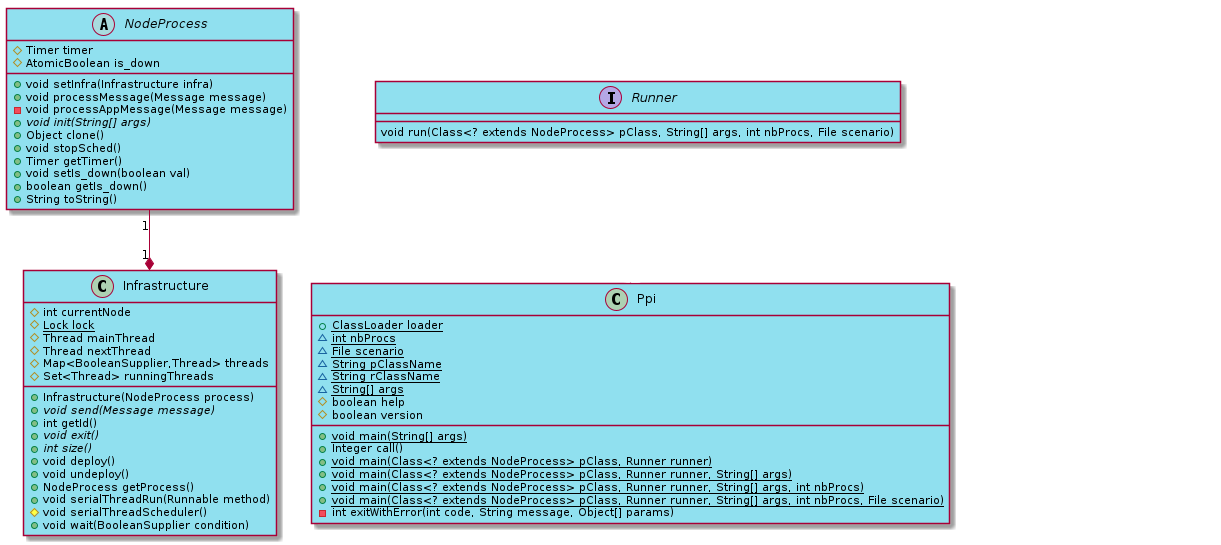
\includegraphics[width=22cm]{uml/generique.png}
					
					\vspace{10mm}
					Nous avons commencé par définir une classe abstraite \verb|NodeProcess| qui représente un processus à exécuter et une autre classe abstraite \verb|Infrastructure| qui contient toutes les méthodes que nous devrons implanter pour les deux API (\verb|MPI| et \verb|PeerSim|), cette classe abstraite permet également d'abstraire l'infrastructure sur laquelle \verb|NodeProcess| est exécutée.
					\newline
					\newline
					Le lancement de \verb|MPI| et de \verb|PeerSim| est complètement différent, c’est pourquoi il est primordial que les deux lancements soient unifiés pour permettre un développement plus rapide et sûr. 
					\newline
					Pour remédier à cette situation, notre solution consiste à créer une interface \verb|Runner| qui permet de lancer les exécutions des deux API avec les mêmes arguments. C'est la classe \verb|Ppi|
					(notre classe \emph{main}) qui se charge d'appeler la méthode \verb|run| du
					\verb|Runner| en lui transmettant ses arguments. La classe \verb|Ppi| prend en
					paramètre le nom de la classe qui hérite de \verb|NodeProcess|, le nom de la classe
					du \verb|Runner| et (facultatifs) des arguments à passer aux processus,
					le nombre de processus ainsi qu’un scénario.
					Selon qu'elle ait été appelée depuis la CLI ou depuis Java, elle se chargera ou
					non d'instancier le \verb|Runner| qu'elle a reçu en paramètre avant de l'exécuter.

					\newpage
					\subsection{Primitives offertes}
					Les primitives mises à disposition correspondent à l'ensemble des méthodes publiques de la classe abstraite \verb|Infrastructure| dont une instance est accessible via la propriété \emph{infra}.
					\newline
					Voici la liste des primitives offertes par notre API générique : 
					\newline
					
					\noindent\begin{minipage}{\linewidth}
					\begin{lstlisting}
public int getId()
					\end{lstlisting}
					Permet de récupérer l'id du processus courant.
					\bigskip
					\end{minipage}

					\noindent\begin{minipage}{\linewidth}
					\begin{lstlisting}
public abstract int size()
					\end{lstlisting}
					Retourne le nombre de n\oe uds dans l'infrastructure.
					\bigskip
					\end{minipage}

					\noindent\begin{minipage}{\linewidth}
					\begin{lstlisting}
public abstract void send(Message message)
					\end{lstlisting}
					Permet d'envoyer un message via Ppi.
					\bigskip
					\end{minipage}

					\noindent\begin{minipage}{\linewidth}
					\begin{lstlisting}
public void wait(BooleanSupplier condition) throws InterruptedException
					\end{lstlisting}
					Attendre tant que la condition passée en paramètre n'est pas évaluée à vrai. Il est recommandé de
					passer une lambda en parammètre.
					\bigskip
					\end{minipage}

					\noindent\begin{minipage}{\linewidth}
					\begin{lstlisting}
public void serialThreadRun(Runnable method)
					\end{lstlisting}
					Afin de garder la propriété de reproductibilité de certaines infrastructures, l'API thread de Java
					ne doit pas être utilisée directement. Cette fonction permet donc de lancer un thread qui sera
					éxécuté en série et dans lequel on peut utiliser la fonction \lstinline{wait} de Ppi décrite ci-dessus.
					\bigskip
					\end{minipage}

					\noindent\begin{minipage}{\linewidth}
					\begin{lstlisting}
public abstract void exit()
					\end{lstlisting}
					Arrête l'éxécution pour le n\oe ud courrant.
					\bigskip
					\end{minipage}

					\subsection{la fonctionalité de \emph{guard}}
					L'un des gros intérêts de notre API est la possibilité de faire des
					\emph{guards}. Il s'agit tout simplement de permettre au processus d'attendre
					sur une condition avant de continuer son exécution. Son utilisation se résume à
					la fonction \lstinline{wait} qui prend un \lstinline{BooleanSupplier}.
					En paramètre, il est donc possible de passer une \emph{lambda}, laquelle sera
					évaluée régulièrement pour vérifier si son résultat est vrai.
					Un fois que c'est le cas l'exécution peut reprendre son cours.

					Cette fonctionnalité est pertinente dans notre cas d'utilisation car c'est de
					cette manière que sont, la plupart du temps, représentés les algorithmes
					distribués.
					Ainsi un algorithme n'a pas besoin d'adaptation de la part du programmer pour
					passer de la conception à la réalisation.

					Pour faire fonctionner cette fonctionalité, un \emph{thread} est lancé pour le
					traitement de chaque événement. De cette manière il nous est possible de
					facilement sauvegarder le contexte d'exécution du process au moment de son appel
					à \lstinline{wait} et également de facilement lui faire reprendre son cours.

					Voici un exemple d'utilisation de la primitive \lstinline{wait} qui permet
					d'afficher une information sur la sortie standard seulement après la réception
					d'un nombre N de message :
					\newpage
					\begin{lstlisting}
public class WaitExample extends NodeProcess {
	public static class ExampleMessage extends Message {}

	private final int N = 2;
	private int msgReceived = 0;

	// affiche "Hello !" sur la console apres N messages recus
	public void helloN() {
		try {
////////////////////////////////////////////////////////////////
////////////////////////// wait ////////////////////////////////
////////////////////////////////////////////////////////////////
			infra.wait(() -> msgReceived >= N);
////////////////////////////////////////////////////////////////
			System.out.println(infra.getId() + " Hello !");
		} catch (InterruptedException e) {
			System.out.println(infra.getId() + " Interrupted while waiting !");
		}
	}

	// gestionnaire de messages
	@MessageHandler
	public void processExampleMessage(ExampleMessage message) {
		int host = infra.getId();
		System.out.printf("%d Received '%s' from %d.\n", host, message.getS(), message.getIdsrc());
		msgReceived++;
		int dest = (host + 1) % infra.size();
		if (host != 0 && msgReceived == 1) {
			infra.send(new ExampleMessage(infra.getId(), dest, "hello"));
			if (host == 2)
				helloN(); // attendre N messages si l'id du noeud est 2
		} else {
			infra.send(new ExampleMessage(infra.getId(), dest, "hello"));
			infra.exit();
		}
	}

	@Override
	public void init(String[] args) {
		if (infra.getId() == 0)
			infra.send(new ExampleMessage(infra.getId(), 1, "hello"));
	}
}
					\end{lstlisting}
					\newpage
					\subsection{La fonctionnalité de scénario}
Notre API permettra aussi de définir des actions ou pannes sur un nœud donné à l'aide d'un scénario prédéfini qui va permettre sont execution,
afin de l'utiliser, il suffit de définir un fichier JSON et d'ajouter le chemin vers ce dernier (nous verrons cela plus en détail en annexe).

\subsubsection{Exemple d'un anneau initialisé par un fichier de scénario}
Ci-dessous nous avons repris l'exemple précédents mais lancé par un appel de fonction lue dans le fichier \verb|fileName|,ainsi que 
la création de ce fichier JSON.
\begin{lstlisting}
public class RingScenarioTest extends NodeProcess{
static String fileName = System.getProperty("user.dir") + "/testJson.json";
public static class RingMessage extends Message {/*Meme que l'exemple precedent*/}
@MessageHandler
public void processRingMessage(RingMessage message) {
int host = infra.getId();
System.out.printf("Noeud "+ host + " a recu " + message.getContent() + " de " + message.getIdsrc());
int dest = (host + 1) % infra.size();
infra.send(new RingMessage(infra.getId(), dest, message.getContent()+1));
infra.exit();
}
public void FirstToSend(){
infra.send(new NodeBreakDownTest.ExampleMessage(infra.getId(),(infra.getId() + 1) % infra.size(), 0));
}
@Override
public void init(String[] args) {/*Rien a metre ici*/}
\end{lstlisting}
Ci-dessou le fichier JSON utiliser il contien l'appele a la fonction FirstToSend sur le neud 0 aprés un délais de 1000 milliseconde
\begin{lstlisting}
{"events":[{"args":[],"FunctionName":"FirstToSend","Node":0,"Delay":1000}]}	
\end{lstlisting}
Ci-dessou une façon de faire pour contruire le fichier JSON (plus de détails en annexe)
\begin{lstlisting}
public static void createJsonTest() {
//exemple de construction d'un fichier scenario
FileWriter filew = new FileWriter(fileName))
JSONObject toWrite = new JSONObject();
JSONArray array = new JSONArray();
int node =  0; // Le node d'id 0 executera la methode FirstToSend
array.add(ProtocolTools.eventBuilder("FirstToSend", node, 1000, new ArrayList<>()));
toWrite.put("events", array);
}
\end{lstlisting}
						\newpage
							
		
						\section{Présentation des deux adapters}
						
						\subsection{L'adapter vers Peersim}
						L'implantation de notre API du côté de \verb|PeerSim| consiste principalement à effectuer un Adapter avec l'API déjà existante de \verb|PeerSim|. Il fallait donc comprendre le fonctionnement des classes de \verb|PeerSim| nécessaires pour faire le lien entre les deux API,  
						et également adapter certaines de nos classes pour \verb|PeerSim|, par exemple rendre \verb|NodeProcess| clonable. 
						\newline
						Ainsi, la classe \verb|PeerSiminfrastructure| fait le lien entre notre API générique et l'API de \verb|PeerSim|.
							\subsubsection{Diagramme UML de l'adapter vers Peersim}
							\hspace*{-1.3cm} 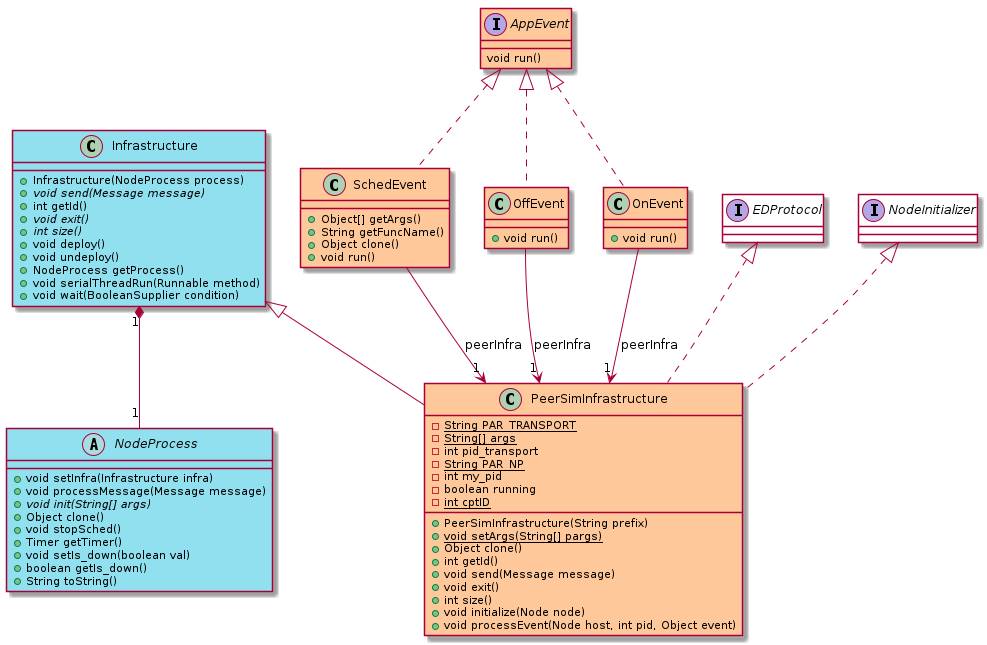
\includegraphics[width=17cm]{uml/peersim1.png}
		
							\hspace*{-3.2cm} 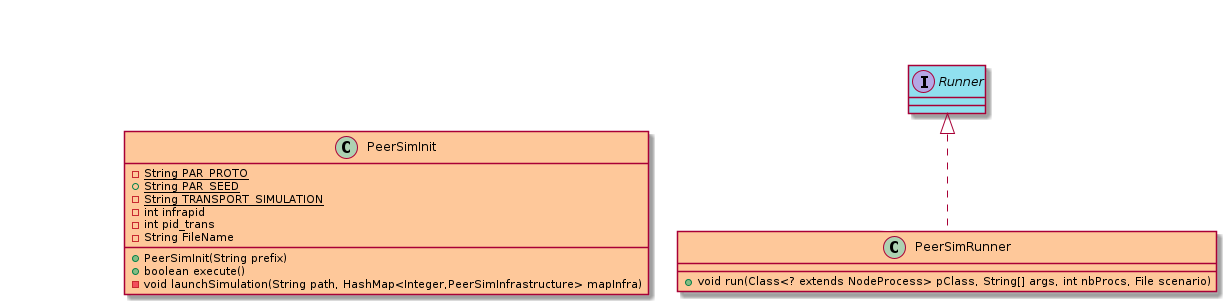
\includegraphics[width=20cm]{uml/peersim2.png}
						
							\subsubsection{Ajout du multithreading}
							L’une des difficultés rencontrées au cours de l’implantation de l’adapter \verb|PeerSim| est de rendre celui-ci \emph{multithreadé} ce qui est une source critique d'indéterminisme.
	En effet, en principe \verb|PeerSim| tourne sur un seul processus et est déterministe. Par conséquent un processus fait à la fois l’aiguillage et exécution des événement de manière séquentielle, nous ne pouvons donc pas implanter une fonctionnalité telle que \emph{wait} qui mettrai le processus en attente. Il a donc fallu voir en détail de comment rendre effectif le \emph{multithread} tout en gardant une cohérence sur les données et surtout le déterminisme. 
	\newline
	\newline
	La solution consiste à avoir un \emph{thread} pricipale qui joue le rôle de l'ordonnanceur et chaque événement sera dédié à un nouveau \emph{thread}.  et parallèlement le \emph{thread} principale se mettra en attente jusqu’à que le \emph{thread} exécutant l’événement finit son exécution ou qu’il se met en attente sur \emph{infra.wait()}.
	\newline
	\newline
	Voici un diagramme de séquence illustrant ceci :

	\vspace{10mm}
	\hspace*{-0.7cm} 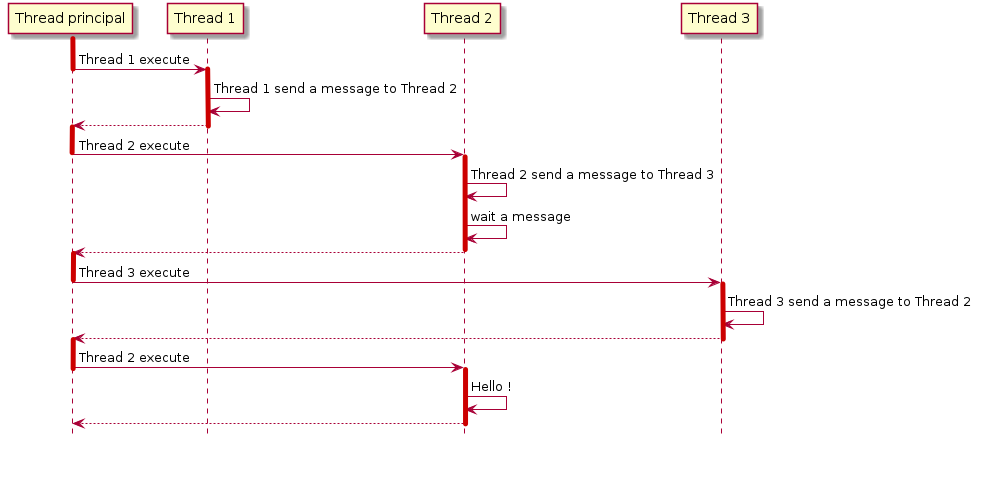
\includegraphics[width=17cm]{uml/diagseq.png}
	\newpage
						\subsubsection{La fonctionnalité de scénario en Peersim}
						\vspace{5mm}
						\hspace*{5cm} 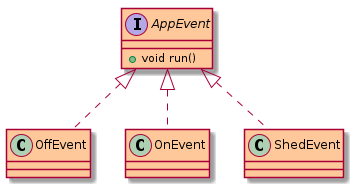
\includegraphics[width=60mm]{uml/scenPuml.png}
						
						\vspace{5mm}
						Peersim ayant déjà une fonctionnalité qui permet de définir un ou plusieurs évènements qui peuvent être définis avec un délai de livraison donné à l'aide de la class \verb|EDSimulator|,
						l'implantation de notre fonctionnalité de scénario vers peersim repose entièrement sur elle.
						En effet la class \verb|EDSimulator| a une fonction \verb|add|
						\begin{lstlisting}
static void add(long delay, java.lang.Object event, Node node, int pid)
						\end{lstlisting}
						qui permet de programmer un événement qui va être délivré sur un nœud donné. 
						\newline
						Nous avons utilisé celle-ci afin de délivrer les évènements définis dans le fichier JSON, au début de l'application si on choisit le runner de \verb|PeersimRunner| , celui-ci va 
						les lire et les ajouter dans la file des évènements de Peersim.
		Pour représenter un événement de l'application, nous avons défini donc une interface \verb|AppEvent|,
						Lorsqu'un le nœud reçoit un tel événement, il exécute la méthode run de l'interface dont les instructions correspondront à l'évènement, par exemple la méthode \verb|run()| la class \verb|SchedEvent| 
						correspondra à l'appel d'une fonction définie par l'utilisateur et  \verb|OnEvent|/\verb|OffEvent| à la fin et début d'une panne.
						Cependant, la notion événementielle n'est pas synchronisé entre notre API et Peersim c'est à dire que si, par exemple, on lance un algorithme lors de l'implémentation de la fonction \verb|init()| celui-ci 
						va s'exécuter indépendamment de la boucle des évènements de peersim, bien sûr ce problème n'existe pas si toutes les instructions sont dans le fichier JSON.
			
			\newpage
			\subsection{L'adapter vers MPI}
			Dans le cas de \verb|MPI|, pour implanter l'adapter, nous avons commencé par implanter un algorithme simple (un anneau). Puis, une fois que nous avons compris l'essentiel de \verb|MPI|, nous avons étendu la classe \verb|Infrastructure|, ainsi la classe \verb|MpiInfrastructure| nous permet de communiquer avec l'API \verb|MPI|. 
			Nous avons, cependant, dû ajouter une boucle afin d'adapter le fonctionnement de \verb|MPI| à celui de \verb|PeerSim|.
				\subsubsection{Diagramme UML de l'adapter vers MPI}
				\vspace{1mm}
				\hspace*{-2.1cm} 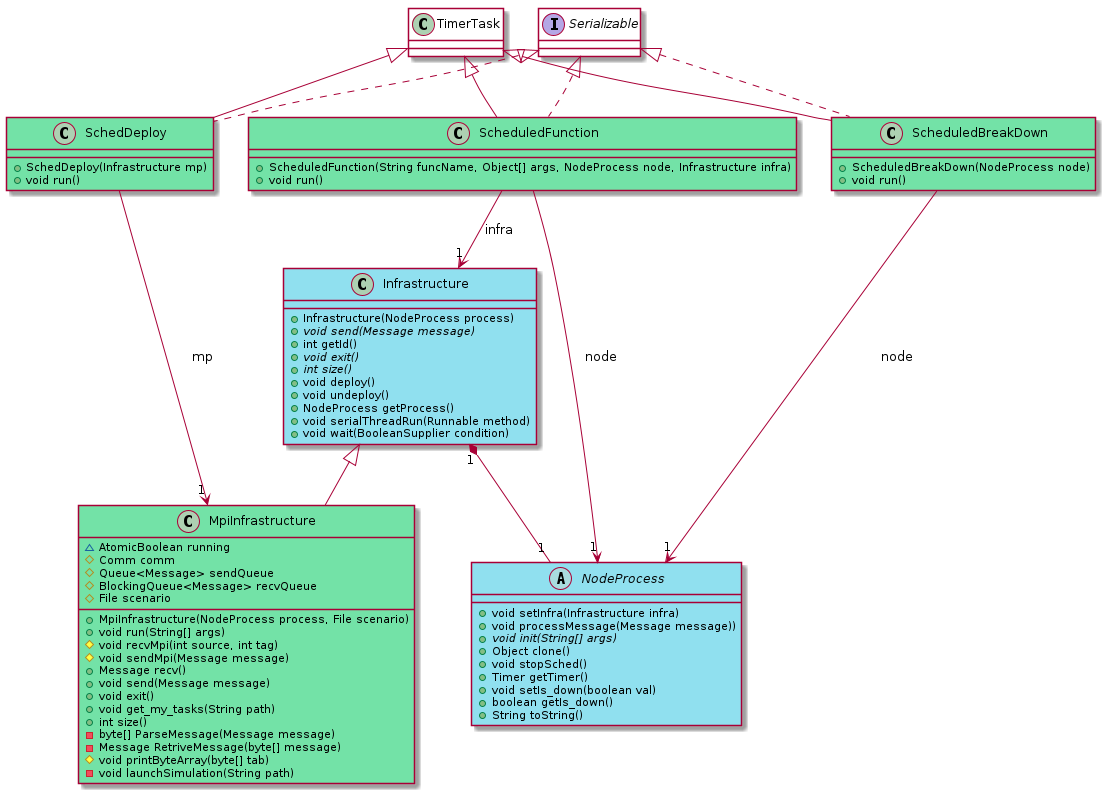
\includegraphics[width=19.5cm]{uml/mpi1.png}
				Le diagramme ci-dessus montre la structure interne de l'implémentation vers MPI, dont le cœur est la classe \verb|MpiInfrastructure|
				et qui se charge de toutes les communications avec MPI.
				\newpage
				\hspace*{-2.3cm} 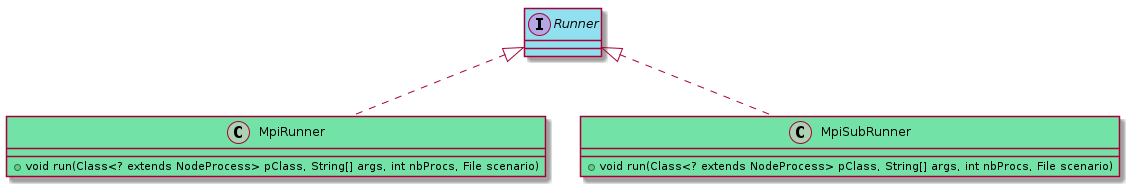
\includegraphics[width=20cm]{uml/mpi2.png}
				Ci-dessus, l'abstraction du lancement MPI afin de permettre à l'utilisateur de lancer l'application sans avoir à utiliser \verb|mpirun|.

				\subsubsection{Passer au modèle événementiel}
				Le modèle de notre API étant événementiel, il a fallu, pour réaliser l'adapter MPI,
				adapter l'infrastrcutre de MPI à ce modèle.

				Nous avont donc ajouté à MPI une boucle d'événements chargée de recevoir et
				d'envoyer des messages MPI. Cette boucle a deux intérêts principaux.
				Le premier est de mettre l'infrastructure MPI au niveau de celle de PeerSim qui
				intègre de base une gestion des événements. En effet grâce à cette boucle il est
				possible de masquer le traitement des récéptions et de déclencher un événement à
				chaque message reçu.

				Son deuxième intérêt est de palier à une faiblesse de MPI, la gestion de threads
				multiples. En effet, MPI dispose de plusieurs modes pour les programmes
				multithreads qui ont chacun leurs inconvénients. Le mode \lstinline{SERIALIZED}
				permet à plusieurs threads d'appeler
				des primitives MPI à condition qu'il n'y en ait qu'un à la fois. Le mode
				\lstinline{MULTIPLE} permet l'appel par plusieurs threads sans restrictions mais
				semble ne pas être stable et n'est pas activé par défaut. Enfin le mode
				\lstinline{FUNNELED} nécessite qu'un seul thread ne fasse des appels MPI.
				Nous avons finalement préféré le mode \lstinline{FUNNELED} au mode
				\lstinline{SERIALIZED} car nous avions déjà un thread dédié au traitement des
				messages.

				\subsubsection{Transmettre des objets Java}
				Pour transmettre des objets Java via MPI nous nous sommes appuiés sur la sérialisation
				intégrée à Java. L'ensemble des propriétés des messages doivent donc être sérialisables.
				Nous transformons ensuite le stream en tableau d'octet que nous envoyons directement
				via MPI. L'utilisation de la fonction \lstinline{}

				\subsubsection{Lancement du processus mpirun}
				Afin de lancer une infrastructure MPI la commande \lstinline{mpirun} doit être lancée
				dans un sous processus. De plus cette commande lancera elle même antant de nouveaux
				processus Java que demandé. Nous avons donc du ajouter un deuxième \lstinline{Runner}
				pour MPI. Le premier permettant de lancer la commande \lstinline{mpirun}, qui elle
				va à nouveau appeler le \lstinline{main} de \lstinline{Ppi} pour chaque processus,
				mais cette faois avec le \lstinline{SubRunner}.
					\newpage
				\subsubsection{Scenario en MPI}
				\vspace{5mm}
				\hspace*{4cm} 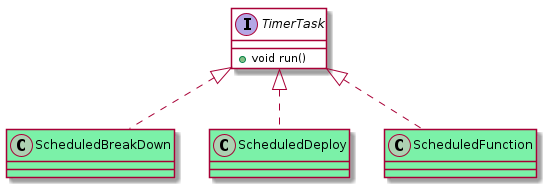
\includegraphics[width=80mm]{uml/scenMPIuml.png}
				
				\vspace{5mm}
				Pour l'implémentation sous MPI nous avons utilisé la classe \verb|Timer| pour planifier un événement sur un noeud donné.
				\newline
				Nous avions commencé par implanter un processus supplémentaire qui ce lançait à chaque demande de simulation et qui se chargeait d'envoyer des 
				messages applicatifs distingués par l'interface \verb|AppMessage|, ainsi chaque processus qui recoit un message étendant cette interface, crée la classe 
				qui étend la classe \verb|TimerTask| et l'insère dans son timer afin qu'elle soit éxécutée en temps voulu.
				\newline
				Cependant cette implémentation c'est révélée être plus compliqueée à mettre en place car elle devait être faite à la construction des processus et fut donc abondonnée.
				\newline
				À la place, dès l'utilisation de l'option scénario avec le MpiRunner, tous les processus reçoivent le chemin vers le fichier JSON, le lisent, et créent les classes correspondantes aux événements.
				\newline
				Afin de modéliser les pannes pour MPI, nous l'avons réalisé au niveau de l'appi générique, ainsi lorsque un nœud est en "panne" il reçoit toujour les message qui lui sont envoyés cependant il les ignorent,
				de ce fait le processus devra être tué malgré tout à la fin de l'exécution de MPI.
				Cependant, il est a noté que cette fonctionnalité n'est pas garantie sur cette API car le réseau et les horloges séparées injectent un nombre d'incertitudes conséquant sur la précision des délais donnés 
				pour les exécution.
		
				
		\newpage
		\section{Plan de validation}

			\subsection{Tests de validation}
			Pour chaque fonctionnalité ajoutée nous ajoutons un test, et nous nous assurons que les tests précédents fonctionnent toujours, ainsi on s'assure que le développement et la fusion d'une autre branche qui aurait été créée en parallèle ne perturbe rien.
			\newline
			\subsubsection{Test du déterminisme lors de l'éxécution sur Peersim}
			Nous avons aussi souhaité vérifier que lorsque du code générique a pour support Peersim, l'éxécution de celui-ci reste bien déterministe, puisque c'est bien une des raisons principales du besoin d'éxécuter du code sur un simulateur au départ. 
Dans le test suivant nous vérifions donc qu'un même code éxécuté avec la même graine aléatoire mène bien à la même trace d'éxécution.\newline
Dans ce cas il s'agit d'un broadcast émis par le noeud d'identifiant 0 à tous les autres. On vérifie par le biais des affichages que l'ordre de réception et de traitement des messages est bien le même
			\begin{lstlisting}
public class BroadcastOrderTest extends RedirectedTest {

	public static class ExampleMessage extends Message {

		private static final long serialVersionUID = 1L;
		private String s;
		public ExampleMessage(int src, int dest, String s) {
			super(src, dest);
			this.s = s;
		}

		public String getS() {
			return s;
		}

	}

	@MessageHandler
	public void processExampleMessage(ExampleMessage message) {
		System.out.printf("%d Received '%s' from %d\n", message.getIddest(), message.getS(), message.getIdsrc());
		infra.exit();
	}

	@Override
	public void init(String[] args) {
		if (infra.getId() == 0) {
			for(int i = 1; i < infra.size(); i++) {
				infra.send(new ExampleMessage(infra.getId(),i, "OrderTest"));
			}
			infra.exit();
		}
	}

	private static final Integer NETWORKSIZE = 10 ;
	private static final String PAR_SIZE = "network.size";

	String outputPeersim;
	@Test
	public void PeersimBroadcastOrderTest() {
		Ppi.main(this.getClass(), new PeerSimRunner(), new String[0], NETWORKSIZE);
		int networkSize=Configuration.getInt(PAR_SIZE);
		int i=0;
		
		outputPeersim=outContent.toString();
		System.out.println(outputPeersim);
		Scanner scanner = new Scanner(outputPeersim);
		String[] expected=new String[networkSize];

		while (scanner.hasNextLine()) {
		  String line = scanner.nextLine();
		  if(line.isEmpty()) {	//Skipping empty output lines
			  continue;
		  }else {
			  String[] results=line.split(" ");
			  System.out.println( "dd"+line);
			  if(i<networkSize-1) { // Initialisation des output expected pour chaque ligne lors du premier experiment
				  
				  expected[i]=results[0]+","+results[2]+","+results[4];
			  
			  }else{	// Comparaison des outputs pour chaque experiment au-dela du premier
				  
				  assertEquals(expected[i%(networkSize-1)],results[0]+","+results[2]+","+results[4]);
			  }
		  }
		i++;
		}
		scanner.close();
	}
}
			\end{lstlisting}

			 \subsubsection{Test d'exclusion mutuelle grâce à l'algorithme de Naimi-Trehel}
			Finalement, nous avons implanté l'algorithme de Naimi-Trehel afin de tester l'ensemble des fonctionnalités, y compris l'ajout du multithreading et notre implementation de la fonctionnalité wait.
			\newline
			Ci-dessous l'algorithme Naimi-Trehel :
			\begin{lstlisting}
public class NaimiTrehel extends NodeProcess {
	Integer father = 0;
	Integer next = null;
	boolean token = false;
	boolean requesting = false;
	int nbCS = 0;
	int nbEnd = 0;// terminaison

	@Override
	public void init(String[] args) {
		if (infra.getId() == father) {
			father = null;
			token = true;
		}
	}

	public void doSomething() {
		infra.wait(() -> requesting == false);
		request();
		infra.wait(() -> token == true);
		cs();
		release();

		// terminaison
		if (nbCS == 2) {
			System.out.printf("%d Had 2 critical sections\n", infra.getId());
			infra.send(new End(infra.getId(), 0));
		}
	}

	public void request() {
		requesting = true;
		if (father != null) {
			infra.send(new Request(infra.getId(), father));
			father = null;
		}
		System.out.printf("%d Requested critical section\n", infra.getId());
	}

	public void cs() {System.out.printf("%d Entered critical section\n", infra.getId()); nbCS++;}

	public void release() {
		requesting = false;
		System.out.printf("%d left critical section\n", infra.getId());
		if (next != null) {
			System.out.printf("%d Send token to %d\n", infra.getId(), next);
			infra.send(new Token(infra.getId(), next));
			token = false;
			next = null;
		}
	}

	@MessageHandler
	public void processRequest(Request request) {
		int host = infra.getId();
		System.out.printf("%d Received request from %d\n", host, request.getIdsrc());
		if (father == null) {
			if (requesting == true) {
				System.out.printf("%d Set %d as next\n", host, request.getIdsrc());
				next = request.getIdsrc();
			} else {
				System.out.printf("%d Send token to %d\n", host, request.getIdsrc());
				infra.send(new Token(host, request.getIdsrc()));
				token = false;
			}
		} else {
			System.out.printf("%d Pass request to %d\n", host, father);
			infra.send(new Request(request.getIdsrc(), father));
		}
		father = request.getIdsrc();
	}

	@MessageHandler
	public void processToken(Token t) {
		int host = infra.getId();
		System.out.printf("%d Received token from %d\n", host, t.getIdsrc());
		token = true;
	}

	//simple class pour differencier les message
	public static class Request extends Message {/*...*/}				
	public static class Token extends Message {/*...*/}
	public static class End extends Message {/*..*/}

	// terminaison
	@MessageHandler
	public void processEnd(End end) {
		if (infra.getId() == 0) {
			nbEnd++;
			if (nbEnd == 5) {
				for (int i = 1; i < 6; i++) {
					infra.send(new End(0, i));
				}
				System.out.printf("%d Called exit\n", infra.getId());
				infra.exit();
			}
		} else {
			System.out.printf("%d Called exit\n", infra.getId());
			infra.exit();
		}
	}
}
			\end{lstlisting}
			
			\subsubsection{Test de scénario incluant une panne}
			Afin de tester les pannes ainsi que les scénarios, nous avons utilisé le test suivant. Celui-ci met en panne un noeud qui ignorera tous les messages reçus, sauf applicatifs, et un second noeud est mis hors-service mais tout de suite remis en ligne.
			\begin{lstlisting}
public class NodeBreakDownTest extends NodeProcess {
	static String fileName = System.getProperty("user.dir") + "/testeJson.json";

	public static class ExampleMessage extends Message {/* ... */}

	@MessageHandler
	public void ExempleMsg(ExampleMessage message) {
		int host = infra.getId();
		System.out.printf("%d Received '%s' from %d\n", host, message.getS(), message.getIdsrc());
		if (host != 0) {
			int dest = (host + 1) % infra.size();
			infra.send(new ExampleMessage(infra.getId(), dest, "Hello"));
			infra.exit();
		} else {
			System.err.println(" not the right path");
		}
	}

	// afin de demander l'arret du processus en panne
	public void End() {
		infra.exit();
	}

	@Override
	public void init(String[] args) {
		if (infra.getId() == 0) {
			infra.send(new ExampleMessage(infra.getId(), 1, "Hello"));
		} else
			Thread.sleep(500);
	}

	// creation du scenario
	@BeforeClass
	@SuppressWarnings("unchecked")
	public static void createJsonTeste() {
		FileWriter filew = new FileWriter(fileName);
		JSONObject toWrite = new JSONObject();
		JSONArray array = new JSONArray();
		// demande de la panne sur le neud 0
		array.add(ProtocolTools.StateBuilder(0, 1000));
		toWrite.put("undeploy", array);
		// dmeande de la panne et l'annulation sur le neud 2
		array = new JSONArray();
		array.add(ProtocolTools.StateBuilder(2, 500));
		toWrite.put("undeploy", array);
		array = new JSONArray();
		array.add(ProtocolTools.StateBuilder(2, 600));
		toWrite.put("deploy", array);
		// arret du process 0 car il ne va jamais appeler @MessageHandler du a la panne
		array.add(ProtocolTools.eventBuilder("End", 0, 5000, new ArrayList<>()));
		toWrite.put("events", array);
		filew.write(toWrite.toString());
	}
}
		\end{lstlisting}

		\subsection{Scénario de validation lors de la soutenance}
Lors de notre soutenance, nous prévoyons de montrer que notre projet passe bien les tests que nous lui avons fixé, et d'expliquer en quoi chacun de ces tests prouve le bon fonctionnement d'une ou plusieurs fonctionnalités de notre projet. Nous nous focaliserons sur les trois tests que nous venons de citer, qui permettent bien de vérifier : 
\begin{itemize}
\item Les fonctionnalités principales, comme l'envoi et la réception de message, l'aiguillage automatique, le multithreading et le wait dans le test \verb|NaimiTrehel| 
\item La conservation du déterminisme lors d'une éxécution sur Peersim dans le \verb|BroadcastOrderTest| 
\item Les fonctionnalités de description de scénario et de panne dans le \verb|NodeBreakdownTest| 
\end{itemize} 
		\newpage
		\section{Conclusion}
			%TODO
			%Piqûre de rappel de ce qu'on disait au début pour montrer qu'on a réussi à le faire 
			\subsection{Objectifs et axes principaux de travail}
			L'objectif premier de ce projet était de réaliser une API permettant de faciliter le test et le déploiement d'applications réparties, puis dans une seconde partie avoir une 
			fonctionnalité permettant de décrire une suite d'évènements. 
			\newline
			Les deux objectifs ont été atteint et notre API permet bien de réaliser ces deux contraintes,
			cependant vu la complexité des API Peersim et MPI sous-jacentes, notre API est loin d'être capable d'exploiter la totalité des fonctionnalités proposées par ces deux platformes.
			\subsection{Axes d'amélioration possibles et ouverture}
			Comme dit précédemment, il existe beaucoup d'axes d'amélioration possible pour notre API, nous avons jugé bon d'en énumérer certaines qui à défaut de temps n'ont pas pu être implémentées.

			\begin{description}
				%\item[Un system qui vérifierait au moment de la compilation l'unicité de @MessageHandler] \hfill \\
				\item[Changer le Scheduler TimerTask par SchedularConfigurer ou @Scheduled.] \hfill \\ TimerTask ne s'est pas révélée être la solution la plus adéquate à notre utilisation et le changer pourrait augmenter la fiabilité de l'exécution du scénario coté Mpi
				\item[Abstraire la totalité du fichier de configuration de Peersim] \hfill \\ une bonne partie du fichier de configuration de Peersim est réécrite par notre application cependant il serait intéressant que l'utilisateur puisse ajouter des configurations sur notre api et les transmettre à Peersim.
				\item[Avertissements sur Peersim] \hfill \\
				Contrairement à MPI, un programme exécuté sur Peersim s'arrête dès le moment où il
				n'y a plus d'événements dans la file. Il serait donc intéressant d'afficher des
				avertissements quand des threads sont encore en train de wait ou bien qu'un n\oe ud
				n'a pas fait appel à \lstinline{exit}. Car si un tel cas se produit, l'application
				ne s'arrêtera pas lors d'un passage à l'infrastructure MPI.
				\item[Optimiser le multithreading] \hfill \\
				En utilisant plus de verrous et en particulier en faisant en sorte que chaque thread
				qui fait appel à \lstinline{wait} attende sur son propre moniteur, il serait possible
				d'optimiser l'exécution.
				\item[Lancer la fonction init dans une SerialThread] \hfill \\
				Ce qui permettrait de pouvoir appeler \lstinline{wait} depuis toutes les fonctions
				du \lstinline{NodeProcess}.
				\item[Ajouter un processeur d'annotation] \hfill \\
				Celui-ci permettrait de valuder qu'un \lstinline{NodeProcess} est bien valide dès
				la compilation de la classe.
				\item[Simplifier l'ajout d'adapter] \hfill \\
				Il est pour le moment asssez compliquer d'ajouter un adapter pour Ppi. Premièrement
				à cause du manque de documentation et deuxièmement à cause d'une API assez mal
				définie par endroits. Il serait possible notemment de refaoctoriser certaines
				portions de code afin de les mettre en commun et ainsi simplifier l'API.
				Notamment en ajoutant des fonctions dans \lstinline{Infrastructure} pour dispatcher
				un événement ainsi que qu'une mise en commun du code de l'exécution de scénario.
			\end{description}
		
		\appendix
		\section{Annexe : répartition des tâches}
			\hspace*{-0.8cm}\begin{tabular}{|c|c|c|}
				\hline
				Tâche & Date d'échéance & Fait par\\[1mm]
				\hline
		  		Se familiariser avec MPI et Peersim & 17/02 & Tous\\[1mm]
				\hline
				Proposer une API générique & 24/02 & Tous\\[1mm]
				\hline
				Implanter l'API pour MPI & 02/03 & Nicolas et Tarik \\[1mm]
				\hline
				Implanter l'API pour PeerSim & 02/03 & Kimmeng et Max \\[1mm]
				\hline
				Créer une classe abstraite Message & 09/03 & Tous\\[1mm]
				\hline
				Unifier le lancement de l'application & 09/03 & Nicolas\\[1mm]
				\hline
				Rédiger le carnet de bord & 16/03 & Tous\\[1mm]
				\hline
				Rédiger le pre-rapport & 23/03 & Tous\\[1mm]
				\hline 
				Implanter l'aiguillage automatique des messages & 23/03 & Tous\\[1mm]
				\hline
				Ajouter la fonctionnalité de description de scenario & 30/03 & Tarik\\[1mm]
				\hline
				Ajouter des fonctionnalités de wait/notify & 25/05 & Nicolas et Kimmeng\\[1mm]
				\hline
				Ajouter des tests plus poussés sur les invariants & 25/05 & Tarik et Max\\[1mm]
				\hline 
				Rédiger le rapport final & 08/06 & Tous\\[1mm]
				\hline
				Soutenance finale & 12/06 & Tous\\[1mm]
				\hline
			\end{tabular}


		\section{Annexe : Prise en main de notre API}

		\subsection{Programmer un algorithme}
		Pour programmer un algorithme à l'aide de Ppi il faut créer une classe qui étend la classe abstraite \lstinline{NodeProcess}. Par la suite l'ensemble des méthodes disponible seront accessibles par l'intermédiaire de la propriété \lstinline{infra}.

		\subsubsection{Etendre le classe \lstinline{NodeProcess}}
		La classe abstraite \lstinline{NodeProcess} contient une methode abstraite \lstinline{init}
		qu'il est nécessaire de redéfinir dans votre classe :
		\begin{lstlisting}
public void init(String[] args)
		\end{lstlisting}
		Cette méthode permet d'initialiser chaque processus à l'aide des arguments qui lui sont
		passés en paramètre. Elle peut être utile comme point de départ d'un algorithme où bien
		simplement pour le paramètrer.
		L'étape suivante sera de créer les différentes classes de message nécessaires au bon
		fonctionnement de votre algorithme.

		\subsubsection{Créer des classes de message}
		Chaque classe de message doit étendre la classe \lstinline{Message} et l'ensemble de son
		contenu doit être \lstinline{Serializable}. De cette manière il sera possible de les envoyer
		via Ppi et de les réceptionner à l'aide de gestionnaires de messages. Il est conseillé de
		créer une classe par type de message applicatif et ainsi de créer un gestionnaire par type
		de message.

		\subsubsection{Définir des gestionnaires de messages}
		Pour définir un gestionnaire de message, rien de plus simple. Ajoutez à votre classe
		héritant de \lstinline{NodeProcess} une fonction pernant en paramètre un objet d'une des
		classes de message que vous venez de définir et ajoutez-y l'annotation
		\lstinline{@MessageHandler} :
		\begin{lstlisting}
@MessageHandler
public void handlerTestMessage(TestMessage msg) {}
		\end{lstlisting}

		Il ne doit y avoir qu'un seul gestionnaire de message par classe de message, sinon le
		premier trouvé sera choisi par Ppi.
		\newline
		\newline
		\newline
		\textbf{NB:} Les méthodes mises à disposition pour l'utilisateur sont décrites dans la partie 2.2.
		Elles sont également consultable en ligne au format javadoc\footnote{\href{https://atlaoui.github.io/ParallelProgramingInterface/org/sar/ppi/Infrastructure.html}{https://atlaoui.github.io/ParallelProgramingInterface/org/sar/ppi/Infrastructure.html}}


		\newpage
		\subsection{Lancer Ppi}
		Un \lstinline{.jar} executable est téléchargeable pour chaque version dans la section \textit{releases}
		de GitHub\footnote{\href{https://github.com/Atlaoui/ParallelProgramingInterface/releases/}{https://github.com/Atlaoui/ParallelProgramingInterface/releases/}}
		ainsi qu'à chaque build sur la branche \lstinline{master} dans les artefacts du
		build\footnote{\href{https://github.com/Atlaoui/ParallelProgramingInterface/actions?query=workflow\%3Abuild+branch\%3Amaster}{https://github.com/Atlaoui/ParallelProgramingInterface/actions?query=workflow\%3Abuild+branch\%3Amaster}}.
		Ce \lstinline{.jar} permettra de compiler vos classes pour ensuite pouvoir les éxécuter.
		\begin{lstlisting}
javac -cp ppi.jar ExampleNodeProcess
		\end{lstlisting}

		\subsubsection{Depuis un shell}
		\noindent\begin{minipage}{\linewidth}
		Ppi dispose d'une interface en ligne de commande dont voici la page d'aide :
		\begin{lstlisting}
Usage: ppi [-hV] [--np=<number>] [-s=<path>] <process-class> <runner-class>
            [<args>...]
       <process-class>     Fully qualified name of the class to use as process
       <runner-class>      Fully qualified name of the class to use as runner
       [<args>...]         Args to pass to the processes
   -h, --help              Display a help message
       --np=<number>       Number of processus in the network
                                Default: 4
   -s, --scenario=<path>   Path to the scenario file
   -V, --version           Print version info
		\end{lstlisting}
		\end{minipage} 
		Et voici un exemple d'utilisation du \lstinline{.jar} executable. Il n'est pas nécessaires
		d'ajouter la classe du processus à exécuter si elle se trouve dans le répertoire courant
		car elle sera dynamiquement chargée :
		\begin{lstlisting}
java -jar ppi.jar ExampleNodeProcess org.sar.ppi.peersim.PeerSimRunner --np=4
		\end{lstlisting}

		\subsubsection{Depuis un programme Java}
		Afin de simplifier l'usage depuis un programme java un ensemble de fonctions
		\lstinline{main} de plus haut niveau que le \lstinline{main} standard a été ajouté. Il est
		composé de la fonction suivante ainsi que de plusieurs déclinaisons de cette fonction
		ommettant chacune un certain nombre de paramètres optionnels :
		\begin{lstlisting}
public static void main(
	Class<? extends NodeProcess> pClass,
	Runner runner,
	String[] args,
	int nbProcs,
	File scenario
) throws PpiException
		\end{lstlisting}
		Dans ce cas d'utilisation il suffit d'exécuter votre classe à l'aide de la commande java en
		ajoutant le \lstinline{.jar} au classpath :
		\begin{lstlisting}
java -cp .:ppi.jar ExampleNodeProcess
		\end{lstlisting}
		\newpage
		\subsection{Décrire un scénario}
		\subsubsection{Introduction}
		La fonctionnalité de description de scénario permet de programmer des événements qui se
		déclencheront au cours de l'éxécution du programme. Un scénario peut être décrit à l'aide
		d'un fichier \lstinline{JSON} contenant les événements et la date à laquelle ils devront
		être appelés, en unités de temps Ppi dont la durée est dépendante de l'infrastructure.

		Sachant que MPI travaille sur des processus distincts et que le temps de transmission des
		messages est inconnu, on ne garantit pas l'exactitude des dates de déclenchement des
		événements.
		\bigskip

			Les événements appellent des fonctions présentes dans votre classe héritant de
			\lstinline{NodeProcess} et il est possible de leur passer des arguments comme on peut le
			voir dans l'exemple suivant.
			\subsubsection{Exemple de scénario}
			\begin{lstlisting}
{
	"undeploy": [
		{
			"node": 0,
			"start": 100
		}
	],
	"events": [
		{
			"args": [
				{ "val": "MonArgument1", "type": "String" },
				{ "val": 4, "type": "Integer" }
			],
			"FunctionName": "End",
			"Node": 1,
			"Delay": 900
		},
		{
			"args": [],
			"FunctionName": "doSomething",
			"Node": 2,
			"Delay": 300
		}
	],
	"deploy": [
		{
			"node": 0,
			"start": 10000
		}
	]
}
			\end{lstlisting}

			Les tableaux Json \lstinline{"undeploy"}, \lstinline{"deploy"} et \lstinline{"events"} contiennent
			les listes des différents appels demandés.
			Chacun contient une liste d'événements, par exemple \lstinline{"undeploy"} est une liste
			d'objet qui définissent \lstinline{"node"}, le noeud concerné et \lstinline{"start"}, la
			date à laquelle le noeud arrêtera de répondre aux messages.
			De la même manière \lstinline{"deploy"} réactive le noeud. Ces listes permettent à elles
			deux de simuler une panne.
			\bigskip

			L'objet \lstinline{"events"} représente une liste d'appel de fonctions utilisateur.
			L'élément \lstinline{"args"} des objets qu'elle contient désigne les arguments qui
			devront être passés à la fonction. Il faudra donc spécifier le type de chaque arguments
			ainsi que sa valeur.

			Notons que les types des arguments acceptés sont les types de base de java.
			Enfin la clé \lstinline{"FunctionName"} représente le nom de la fonction à appeler.
			\bigskip

			Pour aider la construction du fichier de configuration nous proposons les primitives de la class ProtocolTools suivante:
			\newline
			Pour construire un appel de fonction
			\begin{lstlisting}
public static JSONObject eventBuilder(String funcName , int node, long delay, List<Object> args);
			\end{lstlisting}
			Pour construire un évenement deploy ou undeploy 
			\newline
			(dépendra du nom de l'objet qui le contiendra)
			\begin{lstlisting}
public static JSONObject StateBuilder(int node, long start_at);
			\end{lstlisting}

			Enfin, pour lancer l'exécution du scénario, il faut juste ajouter le nombre de processus et le chemin vers le fichier Json au runneur souhaité.
		%\newpage		
		%\subsection{Comment écrire son propre adapter pour un autre support}

		
\end{document}
